\documentclass[a4paper, 12pt]{article}

%opening
\usepackage{amsmath}
\usepackage{enumitem}
\usepackage{tikz}
\usetikzlibrary{calc,fit,trees}

\newcommand{\bd}{\textbf}

% Start: Title configs
\usepackage{titling}
\pretitle{\begin{flushleft}\Large\bfseries}
\posttitle{\par\end{flushleft}}
\preauthor{\begin{flushleft}\Large}
\postauthor{\end{flushleft}}
\predate{\begin{flushleft}}
\postdate{\end{flushleft}}

\title{
    Assignment: First Order Logic\\
    COMP6065001 --- Artificial Intelligence
}
\author{
    \bd{Nama:} Juan Christian \\
    \bd{NIM/Kelas:} 2501994771 / LG01
}
\date{}
% End: Title Configs

\begin{document}

% === Page 1 === %
\maketitle
\section*{Problem}
Given sentences as premise:
\begin{enumerate}
    \item John is a student
    \item John is in the Informatics department
    \item Each Informatics' student must be an engineering student
    \item Mathematic is a difficult lesson
    \item Each engineering student would definitely like Mathematic or hate it
    \item Each student would definitely like a lesson
    \item Students who have never attended difficult lesson certainly do not like the lesson
    \item Peter has never attended the Mathematic lesson
\end{enumerate}
Based on given premises above, please create:

\begin{enumerate}[label=(\alph*)]
    \item FOL
    \item Convert FOL in part a) to CNF
    \item Proof by Resolution, that \bd{Peter hate Mathematic}
\end{enumerate}
\newpage
% === End of Page 1 === %

% === Page 2 === %
\section*{FOL}

Predicates

\begin{itemize}
    \item $S(x)$ where $x$ is a student
    \item $D(x, y)$ where $x$ is in department $y$
    \item $DF(x)$ where $x$ is a difficult lesson
    \item $L(x, y)$ where $x$ likes lesson $y$
    \item $A(x, y)$ where $x$ attend lesson $y$
\end{itemize}
\bd{1. John is a student}
$$
    S(John)
$$
\bd{2. John is in the Informatics department}
$$
    D(John, Informatics)
$$
\bd{3. Each Informatics' student must be an engineering student}
$$
    \forall{x}\ S\left(x\right)\land D\left(x,\ Informatics\right)\Rightarrow D\left(x,\ Engineering\right)
$$
\bd{4. Mathematic is a difficult lesson}
$$
    DF(Mathematic)
$$
\bd{5. Each engineering student would definitely like Mathematic or hate it}
$$
    \forall{x}\ S\left(x\right)\land D\left(x,\ Engineering\right)\Rightarrow L\left(x,\ Mathematic\right)\vee\lnot L\left(x,\ Mathematic\right)
$$
\bd{6. Each student would definitely like a lesson}
$$
    \forall{x}\ S(x) \Rightarrow \exists{y}\ L(x, y)
$$
\bd{7. Students who have never attended difficult lesson certainly do not like the lesson}
$$
    \forall{x}\forall{y}\ S(x) \land DF(y) \land \lnot A(x, y) \Rightarrow \lnot L(x, y)
$$
\bd{8. Peter has never attended the Mathematic lesson}
$$
    \lnot A(Peter, Mathematic)
$$
\newpage
% === End of Page 2 === %

% === Page 3 === %
\section*{Convert FOL in part (a) to CNF}

\bd{1. John is a student}
$$
    S(John)
$$
\bd{2. John is in the Informatics department}
$$
    D(John, Informatics)
$$
\bd{3. Each Informatics' student must be an engineering student}
\begin{align*}
    \forall{x}\ S(x)\land D(x,Informatics)\Rightarrow D(x,Engineering)       \\
    \forall{x}\ \lnot S(x) \lor \lnot D(x,Informatics) \lor D(x,Engineering) \\
    \lnot S(x) \lor \lnot D(x,Informatics) \lor D(x,\ Engineering)
\end{align*}
\bd{4. Mathematic is a difficult lesson}
$$
    DF(Mathematic)
$$
\bd{5. Each engineering student would definitely like Mathematic or hate it}
\begin{align*}
    \forall{x}\ S(x)\land D(x,Engineering)\Rightarrow L(x,Mathematic)\lor \lnot L(x,Mathematic)        \\
    \forall{x}\ \lnot S(x) \lor \lnot D(x,Engineering) \lor L(x,Mathematic) \lor \lnot L(x,Mathematic) \\
    \lnot S(x) \lor \lnot D(x,Engineering) \lor L(x,Mathematic) \lor \lnot L(x,Mathematic)
\end{align*}
\bd{6. Each student would definitely like a lesson}
\begin{align*}
    \forall{x}\ S(x) \Rightarrow \exists{y}\ L(x, y) \\
    \forall{x}\lnot S(x) \lor \exists{y}\ L(x, y)    \\
    \forall{x}\exists{y}\lnot S(x) \lor L(x, y)      \\
    \forall{x}\lnot S(x) \lor L(x, f(x))             \\
    \lnot S(x) \lor L(x, f(x))
\end{align*}
\bd{7. Students who have never attended difficult lesson certainly do not like the lesson}
\begin{align*}
    \forall{x}\forall{y}\ S(x) \land DF(y) \land \lnot A(x, y) \Rightarrow \lnot L(x, y) \\
    \forall{x}\forall{y}\lnot(S(x) \land DF(y) \land \lnot A(x, y)) \lor \lnot L(x, y)   \\
    \forall{x}\forall{y}\lnot S(x) \lor \lnot DF(y) \lor A(x, y) \lor \lnot L(x, y)      \\
    \lnot S(x) \lor \lnot DF(y) \lor A(x, y) \lor \lnot L(x, y)
\end{align*}
\bd{8. Peter has never attended the Mathematic lesson}
$$
    \lnot A(Peter, Mathematic)
$$
\newpage
% === End of page 3 === %
% === Page 4 === %
\section*{Proof by Resolution, that Peter hate Mathematic}
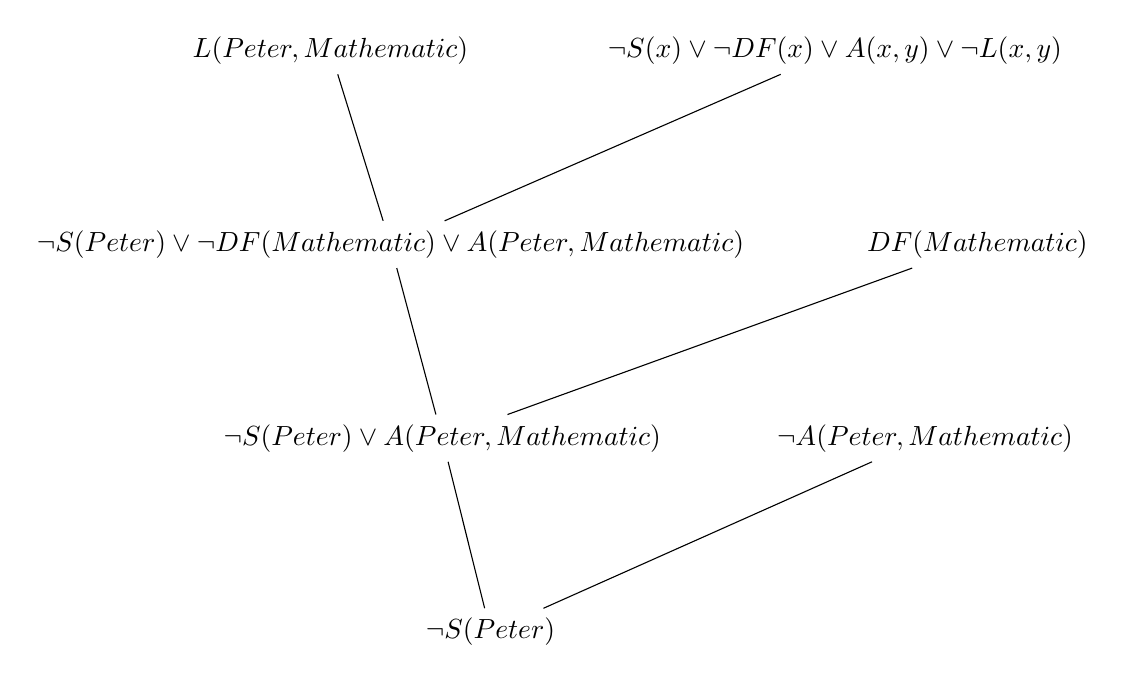
\begin{tikzpicture}[
        grow'=up,
        anchor=west,
        level distance=7em,
        level 1/.style={sibling distance=20em},
        level 2/.style={sibling distance=30em},
        level 3/.style={sibling distance=15em}
    ]
    \node (f) {$\neg S(Peter)$}
    child {
            node(1l) {$\neg S(Peter) \lor A(Peter, Mathematic)$}
            child {
                    node (2ll) {$\neg S(Peter) \lor \neg DF(Mathematic) \lor A(Peter, Mathematic)$}
                    child {node(3lll) {$L(Peter, Mathematic)$}}
                    child {node(3lll) {$\neg S(x) \lor \neg DF(x) \lor A(x, y) \lor \neg L(x,y)$}}
                }
            child { node (2ll) {$DF(Mathematic)$}}
        }
    child { node(1l) {$\neg A(Peter, Mathematic)$} };
\end{tikzpicture}
Therefore, since the resolution tree does not end with a null result. It is proven that the statement "Pether hate mathematic" is \bd{FALSE}.

% === End of page 4 === %
\end{document}